\documentclass[a4paper,14pt]{extarticle}
\usepackage[utf8x]{inputenc}
\usepackage[T1,T2A]{fontenc}
\usepackage[russian]{babel}
\usepackage{hyperref}
\usepackage{indentfirst}
\usepackage{listings}
\usepackage{color}
\usepackage{here}
\usepackage{array}
\usepackage{multirow}
\usepackage{graphicx}
\usepackage{caption}
\usepackage{subcaption}
\usepackage{chngcntr}
\usepackage[fleqn]{amsmath}
\usepackage{amssymb}
\usepackage{pgfplots}
\usepackage{pgfplotstable}
\counterwithin{figure}{section}
\counterwithin{equation}{section}
\counterwithin{table}{section}
\usepackage{tabularx}

%% Поля подписи и даты
\newcommand{\sign}[1][5cm]{%
\makebox[#1]{\hrulefill}
}

\usepackage[left=2cm,right=2cm,
top=2cm,bottom=2cm,bindingoffset=0cm]{geometry}


\begin{document}	% начало документа

\begin{titlepage}	% начало титульной страницы

	\begin{center}		% выравнивание по центру

		\large Санкт-Петербургский Политехнический Университет Петра Великого\\
		\large Институт компьютерных наук и технологий \\
		\large Кафедра компьютерных систем и программных технологий\\[4cm]
		% название института, затем отступ 6см
		
		 \huge Вычислительная математика\\[0.3cm] % название работы, затем отступ 0,5см
		 \large Расчётное задание №2\\[0.1cm]
		 \large Интерполяция\\[8cm]

	\end{center}


	\begin{flushright} % выравнивание по правому краю
		\begin{minipage}{0.35\textwidth} % врезка в половину ширины текста
			\begin{flushleft} % выровнять её содержимое по левому краю

				\large\textbf{Работу выполнил:}\\
				\large Ламтев А.Ю.\\
				\large {Группа:} 23501/4\\
				
				\large \textbf{Преподаватель:}\\
				\large Цыган В.Н.

			\end{flushleft}
		\end{minipage}
	\end{flushright}
	
	\vfill % заполнить всё доступное ниже пространство

	\begin{center}
	\large Санкт-Петербург\\
	\large \the\year % вывести дату
	\end{center} % закончить выравнивание по центру

\thispagestyle{empty} % не нумеровать страницу
\end{titlepage} % конец титульной страницы

\vfill % заполнить всё доступное ниже пространство


\section{Задание}

\begin{displaymath}
f(x) = e^{2 \cdot x} + cos(\pi \cdot x)
\end{displaymath}

\begin{enumerate}

\item Вычислить значения функции в точках $x_0 = 0$, $x_1 = \frac{1}{6}$, $x_2 = \frac{1}{4}$, $x_3 = \frac{1}{2}$

\item Построить интерполяционный полином в форме Лагранжа

\item Построить интерполяционный полином в форме Ньютона

\item Вычислить оценку погрешности для точек $x = \frac{1}{5}$, $x = \frac{1}{3}$

\item Вычислить реальные погрешности интерполяции для этих точек

\item Построить график погрешности для значений на интервале $\Bigl [ 0, \frac{1}{2} \Bigl ]$

\end{enumerate}

\section{Решение}

\begin{table}[H]
	\begin{center}
	\caption{Узлы интерполирования и значения функции в них}
	\renewcommand{\tabcolsep}{1cm}
	\renewcommand{\arraystretch}{2}
		\begin{tabular}{|c|c|c|}
			\hline 
			$k$ & $x_k$ & $f(x_k)$ \\  
			\hline 
			0 & 0 & 2 \\ 
			\hline 
			1 & $\frac{1}{6}$ & 2.261637 \\
			\hline 
			2 & $\frac{1}{4}$ & 2.355828 \\  
			\hline 
			3 & $\frac{1}{2}$ & 2.718281 \\ 
			\hline 
		\end{tabular} 	
		\label{tabular:11}
	\end{center}
\end{table}

\subsection{Построение интерполяционного полинома в форме Лагранжа}

\begin{displaymath}
Q_m(x) = \sum_{k=0}^m \frac{\omega_k(x)}{\omega_k(x_k)} \cdot f(x_k)
\end{displaymath}

\begin{itemize}

\item k = 0:

$\frac{\omega_0(x)}{\omega_0(x_0)} \cdot f(x_0) = \frac{(x - \frac{1}{6}) \cdot (x - \frac{1}{4}) \cdot (x - \frac{1}{2})}{(0 - \frac{1}{6}) \cdot (0 - \frac{1}{4}) \cdot (0 - \frac{1}{2})} \cdot 2 = - 96 \cdot x^3 + 88 \cdot x^2 - 24 \cdot x + 2$

\item k = 1:

$\frac{\omega_1(x)}{\omega_1(x_1)} \cdot f(x_1) = \frac{(x - 0) \cdot (x - \frac{1}{4}) \cdot (x - \frac{1}{2})}{(\frac{1}{6} - 0) \cdot (\frac{1}{6} - \frac{1}{4}) \cdot (\frac{1}{6} - \frac{1}{2})} \cdot 2.261637 = 488.513592 \cdot x^3 + 366.385194 \cdot x^2 + \\[1mm] + 61.064199 \cdot x$

\item k = 2:

$\frac{\omega_2(x)}{\omega_2(x_2)} \cdot f(x_2) = \frac{(x - 0) \cdot (x - \frac{1}{6}) \cdot (x - \frac{1}{2})}{(\frac{1}{4} - 0) \cdot (\frac{1}{4} - \frac{1}{6}) \cdot (\frac{1}{4} - \frac{1}{2})} \cdot 2.355828 = -452.318976 \cdot x^3 + \\[1mm] + 301.545984 \cdot x^2 - 37.693248 \cdot x$

\item k = 3:

$\frac{\omega_3(x)}{\omega_3(x_3)} \cdot f(x_3) = \frac{(x - 0) \cdot (x - \frac{1}{6}) \cdot (x - \frac{1}{4})}{(\frac{1}{2} - 0) \cdot (\frac{1}{2} - \frac{1}{6}) \cdot (\frac{1}{2} - \frac{1}{4})} \cdot 2.718281 = 65.238744 \cdot x^3 - \\[1mm] - 27.182810 \cdot x^2 + 2.718281 \cdot x$

\end{itemize}

\begin{displaymath}
Q_3(x) = \sum_{k=0}^3 \frac{\omega_k(x)}{\omega_k(x_k)} \cdot f(x_k)
\end{displaymath}

\begin{displaymath}
Q_3(x) = 5.433360 \cdot x^3 - 4.022019 \cdot x^2 + 2.089231 \cdot x+2
\end{displaymath}

\subsubsection{Оценка погрешности}

\begin{itemize}

\item $x = \frac{1}{5}$

$\Bigl | \frac{f(x) - Q_3(x)}{f(x)} \Bigl | = \Bigl | \frac{2.300841 - 2.300432}{2.300841} \Bigl | = 1.778531 \cdot 10^{-4}$

\item $x = \frac{1}{3}$

$\Bigl | \frac{f(x) - Q_3(x)}{f(x)} \Bigl | = \Bigl | \frac{2.447734 - 2.450755}{2.447734} \Bigl | = 1.234231 \cdot 10^{-3}$

\end{itemize}

\subsubsection{Вычисление реальной погрешности}

\begin{displaymath}
\epsilon(x) = f(x) - Q_3(x)
\end{displaymath}

\begin{itemize}

\item $x = \frac{1}{5}$

$\epsilon(\frac{1}{5}) = 4.092120 \cdot 10^{-4}$

\item $x = \frac{1}{3}$

$\epsilon(\frac{1}{3}) = -3.021070 \cdot 10^{-3}$

\end{itemize}

\subsubsection{График погрешности}

\begin{figure}[H]
	\begin{center}
		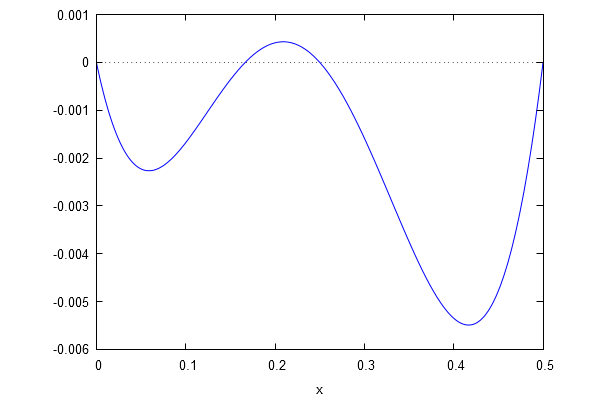
\includegraphics[width=15cm]{image.png}
		\caption{График реальной погрешности $\epsilon(x)$} 
		\label{pic:1}
	\end{center}
\end{figure}

\end{document}
